% MAAI 901 Deep Learning for Visual Data: Deep Learning Project report (group).
% Upload this folder (with figures/) to Overleaf and compile with pdfLaTeX.
\documentclass[11pt,a4paper]{article}
\usepackage[margin=2.2cm]{geometry}
\usepackage[T1]{fontenc}
\usepackage{mathptmx}
\usepackage{graphicx}
\usepackage{booktabs}
\usepackage{amsmath}
\usepackage{etoolbox}
\usepackage[hidelinks]{hyperref}
\patchcmd{\thebibliography}{\section*{\refname}}{}{}{}
\setlength{\parskip}{4pt}

\title{Reading Candlestick Charts with Seven Vision Networks:\\ Direction, Volatility and Drawdown Risk for 50 US Stocks}
\author{Krishna Harsha Tangirala (lead author) \and Mohammed Shahrukh \and Valavala Divya Anu Sri \and Sreeya Tirumalasetti \and Venkata Saisravan Pasam\\[2pt]
\small Master of Applied Artificial Intelligence, University of Wollongong in Dubai\\
\small MAAI 901 Deep Learning for Visual Data, Deep Learning Project (group)}
\date{}

\begin{document}
\maketitle

\begin{center}
\small
GitHub repository: \url{https://github.com/harshatangirala/nexus-alpha-v3-university-of-wollongong-in-dubai}\\
CV dataset (price bars the charts are drawn from): \url{https://drive.google.com/file/d/1Y7wvfpJcjnmXLP79hHTih-jj5pt-muu-/view}\\
Lite dashboard (public, always on): \url{https://nexus-alpha-v3-lite.streamlit.app}\\
Full dashboard (heavy, runs on the author's machine): \url{https://buffalo-deposits-graph-legends.trycloudflare.com}
\end{center}

\section{Executive summary}

We asked whether a deep vision network can read a stock's candlestick charts well enough to forecast three things over the next 5, 10, 20 and 40 trading sessions: the direction of the price (down, sideways or up), how volatile it will be, and whether it will fall more than 10\%. Seven networks were compared on exactly the same rows: a small CNN trained from scratch, ResNet-50, EfficientNet-B0, ConvNeXt-Tiny, ViT-B/16, Swin-T and the classification version of YOLOv8. Each one sees three charts per decision day (weekly, daily and hourly) for 50 large US stocks between October 2016 and August 2026. Every choice was made on 2022--2023 data and frozen with a hash before we opened a locked test set covering January 2024 to August 2026.

On that test the networks showed a small but statistically supported direction signal at 5 and 10 sessions, about +0.03 macro-F1 above a shuffled-label null, and they ranked drawdown risk better than chance at three of four horizons. Six of the twelve pre-registered tests passed after Holm correction. Against simple numerical baselines the picture splits: charts help with direction, while trailing volatility and technical indicators clearly beat them on volatility and drawdown. We trace that gap to a design decision, namely scaling each chart to its own high and low. The models run behind a working Streamlit dashboard that reads TradingView screenshots and redraws them in the training format.

\section{Introduction and problem definition}

Retail investors look at candlestick charts every day, and charting platforms now sell pattern recognition as an AI feature. Whether a network actually extracts forward-looking information from those pictures is an empirical question that marketing does not answer. Jiang, Kelly and Xiu showed that a CNN trained on simple price images can predict US stock returns \cite{jkx2023}, but most follow-up work uses one architecture, one timeframe and one target, and rarely tests the result on a period that was hidden until the end.

Our problem statement is therefore narrow and testable. Given the weekly, daily and hourly charts of a stock on a decision day, can a vision model forecast (a) the three-class direction of the price after $h$ sessions, (b) the log realised volatility over those sessions and (c) the event of a fall of more than 10\% below the decision-day close, for $h \in \{5,10,20,40\}$? We also wanted to know which family of architecture does best, whether fine-tuning beats frozen ImageNet features, whether the answer changes by sector, and whether combining networks helps.

The relevance goes beyond finance. Charts are an unusual visual domain: synthetic, low-texture images where the useful signal sits in geometry and scale and there are no objects to find. Testing modern vision backbones there, under strict leakage control, says something about how far ImageNet features transfer.

\section{Related work and background}

Image-based return prediction started with CNNs applied to bar charts \cite{sezer2019} and gained attention with the large-scale study of Jiang et al. \cite{jkx2023}, who found that the signal was strongest for small stocks and short horizons. Ho and Huang combined candlestick images with sentiment \cite{ho2021}. These studies share two habits we wanted to avoid: a single architecture and a test period that was visible during model development.

The seven networks span the main design ideas of the last decade. ResNet introduced residual connections \cite{he2016}, EfficientNet scales depth, width and resolution together \cite{tan2019}, and ConvNeXt modernises the convolutional design with ideas borrowed from transformers \cite{liu2022convnext}. ViT treats an image as a sequence of $16\times16$ patches \cite{dosovitskiy2021}, while Swin restricts attention to shifted local windows \cite{liu2021swin}. YOLO was built for real-time detection \cite{redmon2016}; we use the classification backbone of YOLOv8 \cite{jocher2023} because chart patterns are often described as objects. For volatility, the HAR model of Corsi \cite{corsi2009} is the standard benchmark, which is why it appears among our baselines. Calibration follows Guo et al. \cite{guo2017}, and corruption robustness follows Hendrycks and Dietterich \cite{hendrycks2019}.

\section{Dataset description}

The universe holds 50 large US stocks, ten in each of five sectors: Information Technology, Financials, Health Care, Consumer Discretionary and Communication Services. Seven names from the original brief were replaced because no verified ten-year hourly history existed for them (for example AVGO by TXN and GOOGL by GOOG). The bars start from a public 1-minute dataset on Hugging Face. We cleaned it, corrected five split dates against Yahoo Finance and aggregated it into regular-hours hourly, daily and weekly bars, split-adjusted but not dividend-adjusted. Occasional daily gaps and the months from March 2026 onward come from Yahoo Finance, and the data end on 9 October 2026. A SHA-256 manifest pins the exact files, so a rerun reads identical inputs.

Sectors were balanced on purpose. With ten stocks each, no sector can dominate the pooled metrics, and we can ask whether one network suits one sector better than another. The price of that choice is breadth: these are large, liquid survivors, and the original image-prediction literature found most of its signal in small companies.

One row is one stock on one decision day. Table~\ref{tab:data} shows how the 64,550 rows divide into time blocks and how the 20-session labels are balanced. Each row carries three images, so the image set holds 193,650 charts (9.72 GB at $224\times224$ pixels).

\begin{table}[h]
\centering
\caption{Time blocks, row counts and 20-session label balance (share of rows).}
\label{tab:data}
\begin{tabular}{lrrrrr}
\toprule
Block & Rows & DOWN & SIDEWAYS & UP & Fall $>$10\% \\
\midrule
Train, Oct 2016 to Dec 2020 & 51,250 & 0.223 & 0.401 & 0.376 & 0.141 \\
Inner, 2021 (early stopping) & 2,150 & 0.220 & 0.397 & 0.383 & 0.093 \\
Validation, 2022--2023 & 4,600 & 0.314 & 0.387 & 0.299 & 0.237 \\
Locked test, Jan 2024 to Aug 2026 & 6,550 & hidden & hidden & hidden & hidden \\
\bottomrule
\end{tabular}
\end{table}

Label thresholds depend on each stock's own volatility. A move counts as SIDEWAYS when the log return over $h$ sessions stays inside $\pm 0.5\,\sigma\sqrt{h}$, where $\sigma$ is the stock's own trailing daily volatility. Volatility is the log of realised volatility computed from hourly bars, and the drawdown label is 1 when the price drops more than 10\% below the decision-day close at any point in the window. The validation block contains the 2022 bear market, which shows in its higher DOWN share and drawdown rate.

\section{Data pre-processing and augmentation}

Charts are drawn from the bars by our own renderer, so every image follows one exact format (Fig.~\ref{fig:inputs}). The weekly view shows 52 candles, the daily view 63 and the hourly view 70, each with a volume strip underneath, in a five-colour palette with no axes, dates or text. Each chart is scaled vertically to its own high and low. That choice keeps the shape of the price path, and as Section~\ref{sec:results} shows, it also removes the absolute level of volatility from the picture.

\begin{figure}[h]
\centering
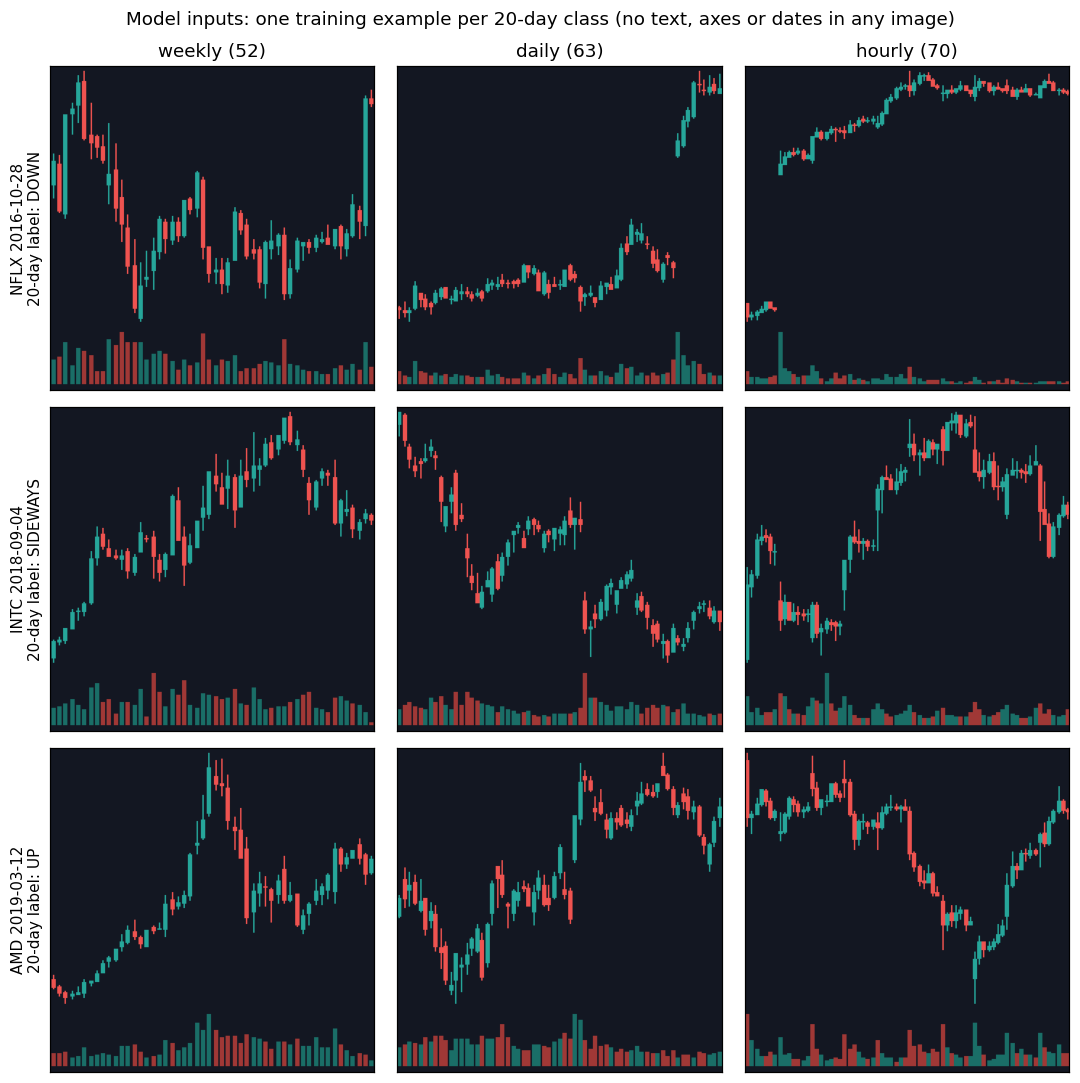
\includegraphics[width=0.62\textwidth]{figures/chart_gallery.png}
\caption{Model inputs for three training rows, one per 20-session class. Each row is a stack of weekly, daily and hourly charts.}
\label{fig:inputs}
\end{figure}

Rising candles are teal, falling ones red, and the volume bars use darker shades of the same two colours. Images are stored as palette indices in 8-bit arrays and turned into RGB tensors on the GPU at training time, which kept the full set of 193,650 images within 9.72 GB. Rendering is deterministic, so any row can be redrawn byte for byte from its bars.

Leakage control mattered more than any modelling choice. Blocks are separated by a 40-session purge so that no label window overlaps the next block, every row uses only bars that closed before the decision time, and seven automated checks (for example that test labels stay hidden and that no stock-date repeats) had to pass before training began.

Augmentation had to respect chart semantics. Horizontal flips would reverse time and vertical flips would turn rallies into crashes, so neither was used. We applied a small vertical rescale, cropping of the oldest bars, brightness changes and Gaussian noise. Images were normalised with each backbone's ImageNet statistics.

\section{Model architecture and implementation}

All seven networks share one wrapper. A single backbone processes the weekly, daily and hourly images separately, the three feature vectors are concatenated, and a multi-task head (layer normalisation, dropout of 0.2, a 512-unit hidden layer with GELU) produces, for each of the four horizons, three direction logits, one volatility value and one drawdown logit. Sharing the backbone across views keeps the parameter count low and lets the head weigh the timeframes.

\begin{table}[h]
\centering
\caption{The seven networks: size, compute per decision row (three views) and learning rate kept by the probe.}
\label{tab:models}
\begin{tabular}{lrrrr}
\toprule
Network & Params (M) & GFLOPs & Learning rate & Train (min) \\
\midrule
Custom CNN, scratch (JKX-style) & 3.39 & 10.22 & $1\times10^{-3}$ & 1.57 \\
ResNet-50 & 26.68 & 24.53 & $3\times10^{-4}$ & 4.92 \\
EfficientNet-B0 & 5.99 & 2.31 & $2\times10^{-4}$ & 5.52 \\
ConvNeXt-Tiny & 29.02 & 26.73 & $1\times10^{-4}$ & 3.88 \\
ViT-B/16 & 86.99 & 105.38 & $2\times10^{-5}$ & 5.36 \\
Swin-T & 28.71 & 26.94 & $1\times10^{-4}$ & 4.92 \\
YOLOv8s-cls & 7.07 & 4.58 & $3\times10^{-4}$ & 2.05 \\
\bottomrule
\end{tabular}
\end{table}

Six backbones start from ImageNet weights through the timm library, and YOLOv8s-cls comes from Ultralytics. The custom CNN follows the Jiang et al. design with wide vertical filters, widened to four blocks for $224$-pixel inputs, and is trained from scratch as the academic baseline. Table~\ref{tab:models} lists sizes and compute. The whole pipeline is a single Colab notebook written in PyTorch, built from 27 readable source files kept in the repository.

The deployed system averages the three networks that scored best on validation for each target, blends in the text models of our companion NLP study when the stock filed with the SEC in the last five sessions, re-calibrates the result, and turns the 20-session forecasts into a Monte Carlo price cone of 4,000 paths. In the dashboard a user pastes TradingView screenshots; the app reads the price axis and candles from the pixels (median price error 0.08\% on 66 real screenshots), redraws the three charts in the training format and runs the networks.

\section{Training strategy and evaluation}

Every network was fine-tuned end to end with AdamW, a warm-up followed by cosine decay, bfloat16 mixed precision and batches of 64 rows, for at most six epochs with early stopping on the 2021 block. A short probe on a training subsample chose between two learning rates per network. Five of the seven networks reached their lowest early-stopping loss after the first epoch (Fig.~\ref{fig:curves}), so the results describe short, early-stopped fine-tuning. Probabilities were calibrated on 2021 only, with temperature scaling for direction, Platt scaling for drawdown and a linear map for volatility.

\begin{figure}[h]
\centering
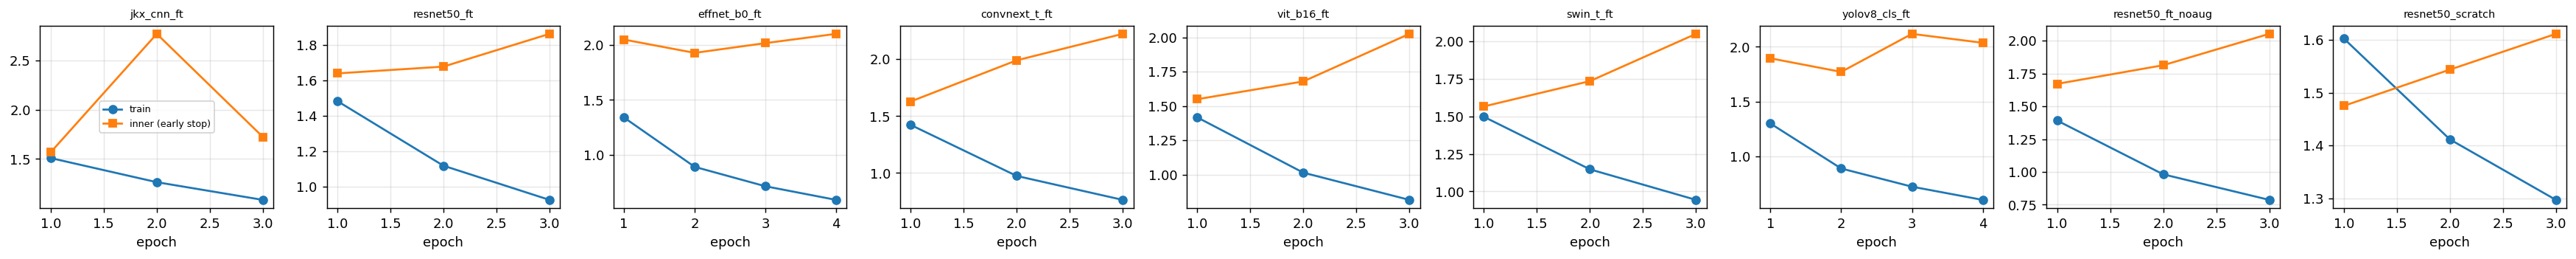
\includegraphics[width=\textwidth]{figures/cv_training_curves.png}
\caption{Training and early-stopping loss per epoch for the seven networks.}
\label{fig:curves}
\end{figure}

The primary metrics were macro-F1 for direction, R-squared for volatility and ROC-AUC for drawdown. Plain accuracy was avoided because always predicting SIDEWAYS already scores about 42\%. Direction skill is macro-F1 minus that of a null model that shuffles labels within each month, so class shares stay the same but the link to the future is broken. Intervals come from a paired month-block bootstrap \cite{kunsch1989}, which respects the dependence between days, and the twelve tests of each hypothesis family were Holm-corrected \cite{holm1979}. Two numerical baselines set a harder bar than chance: \texttt{baseline\_simple} (momentum for direction, HAR for volatility, a trailing-volatility logistic model for drawdown) and \texttt{tech\_gbm}, a LightGBM model on 20 technical indicators. The stronger of the two was chosen on validation for each target.

\section{Results and analysis}
\label{sec:results}

\begin{table}[h]
\centering
\caption{Locked test (H1): skill of the validation-chosen network over the uninformed benchmark, with 95\% bootstrap intervals. Direction skill is macro-F1 above the shuffled null; volatility is R-squared; drawdown is AUC minus 0.5.}
\label{tab:h1}
\begin{tabular}{llrrc}
\toprule
Task & Network & Skill & 95\% interval & Holm-supported \\
\midrule
Direction 5 & ConvNeXt-T & +0.032 & [0.019, 0.043] & yes \\
Direction 10 & ConvNeXt-T & +0.030 & [0.015, 0.046] & yes \\
Direction 20 & ConvNeXt-T & +0.027 & [0.006, 0.047] & no (p = 0.06) \\
Direction 40 & EfficientNet-B0 & +0.012 & [$-$0.006, 0.030] & no \\
Volatility 5 & Swin-T & +0.084 & [0.032, 0.122] & yes \\
Volatility 10 & ViT-B/16 & +0.032 & [$-$0.046, 0.089] & no \\
Volatility 20 & ViT-B/16 & $-$0.029 & [$-$0.135, 0.051] & no \\
Volatility 40 & YOLOv8s-cls & $-$0.182 & [$-$0.339, $-$0.072] & no \\
Drawdown 5 & Swin-T & +0.105 & [0.059, 0.164] & yes \\
Drawdown 10 & ResNet-50 & +0.086 & [0.054, 0.126] & yes \\
Drawdown 20 & EfficientNet-B0 & 0.000 & [$-$0.033, 0.033] & no \\
Drawdown 40 & ViT-B/16 & +0.040 & [0.014, 0.067] & yes \\
\bottomrule
\end{tabular}
\end{table}

Table~\ref{tab:h1} gives the confirmatory result: six of twelve tests passed. Direction is the clearest case. ConvNeXt-Tiny was the validation choice for three of the four horizons and stayed the best direction network on the test in every sector. Its gain is small, which fits a three-class label whose sideways band moves with each stock's volatility.

Fig.~\ref{fig:bench} puts the networks next to the numerical baselines. On direction the top-3 chart ensemble scores a higher macro-F1 than either baseline at every horizon. We do not read that as a large win, because the baselines predict mostly one class, which macro-F1 punishes. A ResNet-50 probe trained on shuffled labels also beats the baselines on macro-F1 in three of four tasks. Judged fairly, each model against its own shuffled null, the chart network is better at 5 sessions (+0.024, interval 0.007 to 0.039) and level with the baselines at 10, 20 and 40. On volatility and drawdown the order reverses: \texttt{tech\_gbm} reaches an R-squared of 0.37 at 5 sessions against 0.13 for the chart ensemble, and the simple drawdown model reaches an AUC of 0.69 against 0.62.

\begin{figure}[h]
\centering
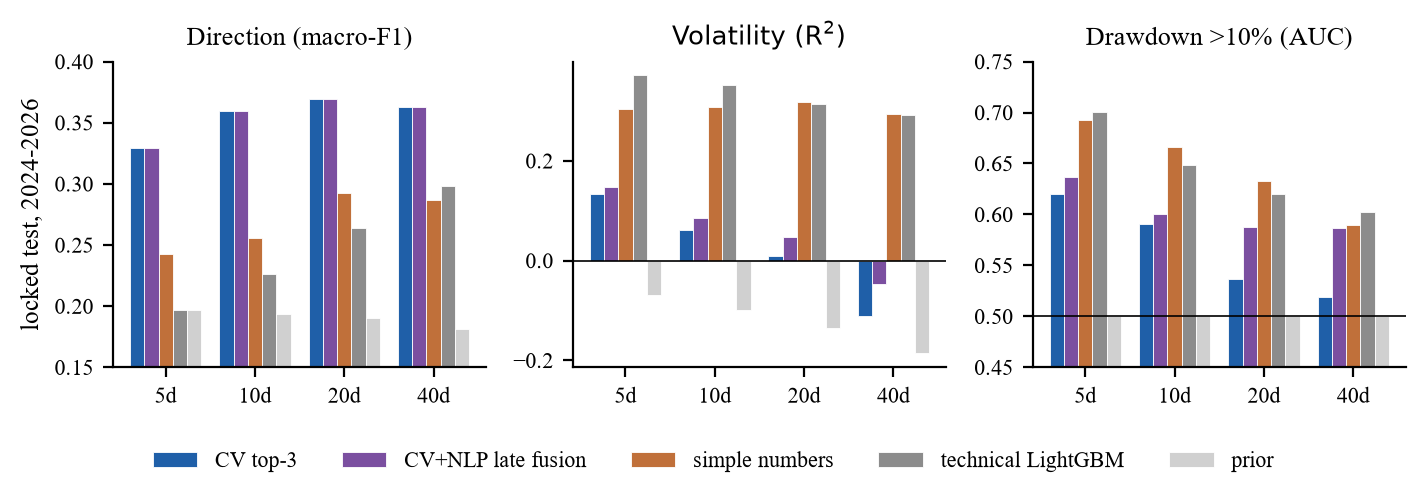
\includegraphics[width=\textwidth]{figures/fig_benchmarks_test.png}
\caption{Locked-test primary metrics for the top-3 chart ensemble, the chart and text fusion, the two numerical baselines and the prior.}
\label{fig:bench}
\end{figure}

The ablations explain much of this. Removing the vertical-rescale augmentation changed volatility R-squared on validation by 0.135 in favour of the un-augmented model, and the per-chart scaling hides how large the candles are in absolute terms. A chart that always fills its frame cannot tell a calm month from a wild one. Fine-tuning beat frozen features in 9 of 18 network-target tests on the locked test (ConvNeXt-T, ViT-B/16 and Swin-T gained most), while EfficientNet-B0 got worse on all three targets, so full fine-tuning on noisy financial labels is not a safe default. ImageNet initialisation beat random initialisation for ResNet-50 on direction (+0.035 macro-F1).

Fig.~\ref{fig:nets} shows every network on the test. The validation winner, ViT-B/16, ranked third on the test, behind Swin-T and ConvNeXt-T; validation covered a bear market and the test a strong rally, so single-model rankings shift with the regime. Averaging the top three per target was the steadier choice, and combinations of two or three networks beat the best single network in 5 of 12 tasks without losing anywhere. Model rankings depended on the sector for volatility and drawdown (permutation p of 0.015 and 0.005) but not for direction.

\begin{figure}[h]
\centering
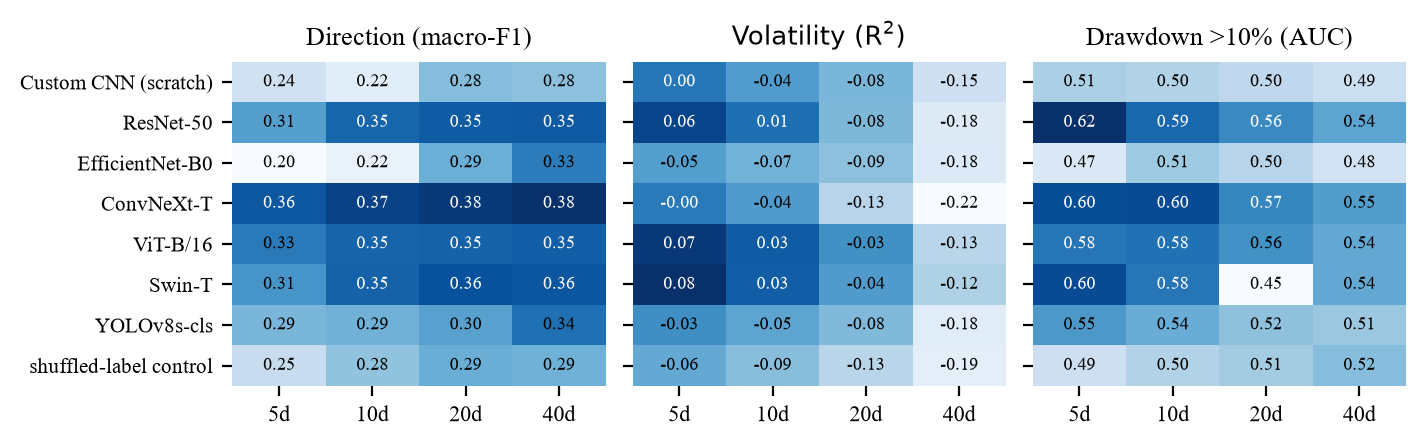
\includegraphics[width=\textwidth]{figures/fig_cv_networks_test.png}
\caption{Locked-test primary metric of each fine-tuned network and of the shuffled-label control.}
\label{fig:nets}
\end{figure}

Two further checks shaped the dashboard. Occlusion showed that the weekly chart moves the predictions most and the hourly chart least. A light-theme rendering lowered ResNet-50's 20-session macro-F1 by 0.16 on validation, while JPEG compression, blur and noise changed little, which is why the app redraws every screenshot in the training style instead of feeding it raw. Finally, the drawdown probabilities rank risk but do not set its level well: their Brier skill against a constant forecast is between $-0.046$ and $-0.015$, so the dashboard presents them as relative risk.

The secondary metrics tell the same story from another angle. At 5 sessions the plain accuracy of ConvNeXt-T is 0.416 against 0.420 for always predicting SIDEWAYS, yet its balanced accuracy is higher by 0.036 on average across horizons. The gain therefore lies in catching the DOWN and UP moves that a majority-class model never calls, which is exactly what macro-F1 rewards.

We also ran the ready-made YOLOv8 chart-pattern detector zero-shot on the weekly charts. Head-and-shoulders, double tops and double bottoms were found on many rows, but the average 20-session return barely differed between rows with and without a pattern (for W-bottoms, 0.9\% against 1.5\%). Named patterns did not add a usable signal here, which is why the dashboard labels its candlestick patterns as descriptive only.

The recipe the dashboard runs was scored on the locked test like any other model. It beat its uninformed benchmark in 9 of 12 tasks after Holm correction: all four direction horizons, 5-session volatility and all four drawdown horizons. The Monte Carlo cone built from its forecasts was checked on the test as well. With the width factor of 1.25 chosen on validation, the nominal 80\% and 90\% ranges contained 82.6\% and 90.8\% of the realised 20-session returns.

\section{Challenges and mitigation}

The first challenge was look-ahead bias. A single leaked label would have inflated every number, so the test block sat in a hashed vault, every opening of it was logged, and the purge and seven leakage checks ran before any training. Analyses added after the test was opened are labelled post-hoc throughout.

The second was an easy metric giving a flattering answer. Raw macro-F1 against one-class baselines made the charts look strong, and the shuffled-label control exposed the problem. We moved to skill over each model's own null and report the smaller number.

The third was a mismatch between training images and what users upload. Real screenshots differ in colours, fonts and indicators, and the robustness test showed how much a theme change can hurt. The dashboard therefore reads the candles and prices from the screenshot and redraws them; on 66 real TradingView images the median price error was 0.08\%.

The fourth was a regime shift between selection and testing. Validation held the 2022 bear market, with a 20-session drawdown rate of 23.7\%, while the test period was a strong rally. A model picked as the single best on validation can fall back on such a test, and ViT-B/16 did. We responded by deploying the average of the three best networks per target and by reporting test ranks next to validation ranks, so the reader can see the shift.

The fifth was compute and instability. Large networks trained for long overfitted the training block, so we kept early stopping short, chose learning rates with a probe and reported the epoch-1 behaviour openly. The full confirmatory run took about 4.2 GPU-hours on a single data-centre GPU in Colab.

\section{Conclusion}

Seven vision networks read the same leakage-controlled charts of 50 US stocks. They carry a real but small direction signal at short horizons, with ConvNeXt-Tiny the most reliable direction model, and they rank drawdown risk better than chance. They do not beat simple numbers on volatility or drawdown, and we can point to why: images scaled to their own range lose the risk level that a trailing-volatility number states directly. For practitioners the lesson is to pair chart models with the absolute numbers instead of replacing them. A pre-registered follow-up will test a chart encoding that keeps the volatility scale, five seeds per network and a forward test period starting in December 2026.

\section{References}

\begin{thebibliography}{99}

\bibitem{jkx2023} J. Jiang, B. Kelly, and D. Xiu, ``(Re-)Imag(in)ing price trends,'' \emph{The Journal of Finance}, vol. 78, no. 6, pp. 3193--3249, 2023.

\bibitem{sezer2019} O. B. Sezer and A. M. Ozbayoglu, ``Financial trading model with stock bar chart image time series with deep convolutional neural networks,'' \emph{Intelligent Automation \& Soft Computing}, vol. 26, no. 2, pp. 323--334, 2019.

\bibitem{ho2021} T.-T. Ho and Y. Huang, ``Stock price movement prediction using sentiment analysis and candlestick chart representation,'' \emph{Sensors}, vol. 21, no. 23, p. 7957, 2021.

\bibitem{he2016} K. He, X. Zhang, S. Ren, and J. Sun, ``Deep residual learning for image recognition,'' in \emph{Proc. IEEE CVPR}, 2016, pp. 770--778.

\bibitem{tan2019} M. Tan and Q. Le, ``EfficientNet: Rethinking model scaling for convolutional neural networks,'' in \emph{Proc. ICML}, PMLR 97, 2019, pp. 6105--6114.

\bibitem{liu2022convnext} Z. Liu, H. Mao, C.-Y. Wu, C. Feichtenhofer, T. Darrell, and S. Xie, ``A ConvNet for the 2020s,'' in \emph{Proc. IEEE CVPR}, 2022, pp. 11976--11986.

\bibitem{dosovitskiy2021} A. Dosovitskiy \emph{et al.}, ``An image is worth 16x16 words: Transformers for image recognition at scale,'' in \emph{Proc. ICLR}, 2021.

\bibitem{liu2021swin} Z. Liu \emph{et al.}, ``Swin Transformer: Hierarchical vision transformer using shifted windows,'' in \emph{Proc. IEEE ICCV}, 2021, pp. 10012--10022.

\bibitem{redmon2016} J. Redmon, S. Divvala, R. Girshick, and A. Farhadi, ``You only look once: Unified, real-time object detection,'' in \emph{Proc. IEEE CVPR}, 2016, pp. 779--788.

\bibitem{jocher2023} G. Jocher, A. Chaurasia, and J. Qiu, ``Ultralytics YOLOv8,'' software, 2023. [Online]. Available: \url{https://github.com/ultralytics/ultralytics}

\bibitem{corsi2009} F. Corsi, ``A simple approximate long-memory model of realized volatility,'' \emph{Journal of Financial Econometrics}, vol. 7, no. 2, pp. 174--196, 2009.

\bibitem{guo2017} C. Guo, G. Pleiss, Y. Sun, and K. Q. Weinberger, ``On calibration of modern neural networks,'' in \emph{Proc. ICML}, PMLR 70, 2017, pp. 1321--1330.

\bibitem{hendrycks2019} D. Hendrycks and T. Dietterich, ``Benchmarking neural network robustness to common corruptions and perturbations,'' in \emph{Proc. ICLR}, 2019.

\bibitem{kunsch1989} H. R. Künsch, ``The jackknife and the bootstrap for general stationary observations,'' \emph{The Annals of Statistics}, vol. 17, no. 3, pp. 1217--1241, 1989.

\bibitem{holm1979} S. Holm, ``A simple sequentially rejective multiple test procedure,'' \emph{Scandinavian Journal of Statistics}, vol. 6, no. 2, pp. 65--70, 1979.

\end{thebibliography}

\section{Links to GitHub repo and demo}

\begin{itemize}
\item GitHub repository (code, notebook, result tables, dashboard): \url{https://github.com/harshatangirala/nexus-alpha-v3-university-of-wollongong-in-dubai}
\item CV dataset, price bars for the 50 stocks (public Google Drive): \url{https://drive.google.com/file/d/1Y7wvfpJcjnmXLP79hHTih-jj5pt-muu-/view}
\item All project data, including the SEC filings used by the language models: \url{https://drive.google.com/drive/folders/13rokT8OX1MgZQpzTRLeyvDq-FVdgraSh}
\item Lite dashboard on Streamlit Community Cloud (public): \url{https://nexus-alpha-v3-lite.streamlit.app}. The full dashboard loads 13 networks (2.9 GB of weights, about 5 GB of memory), which is too heavy for free hosting, so the lite version shows the architecture, the evidence and precomputed full-model results for four stocks.
\item Full dashboard (runs on the author's machine through a tunnel, available during demonstrations): \url{https://buffalo-deposits-graph-legends.trycloudflare.com}
\end{itemize}

\textbf{Team contributions.} Krishna Harsha Tangirala defined the research question and the seven-network design, chose the targets and horizons, ran every Colab execution of the notebook, reviewed each result and audit, decided which post-hoc checks to add and directed the dashboard. [Mohammed Shahrukh: role and contribution.] [Valavala Divya Anu Sri: role and contribution.] [Sreeya Tirumalasetti: role and contribution.] [Venkata Saisravan Pasam: role and contribution.]

\textbf{Use of generative AI.} Following the UOW guidance on acknowledging GenAI, we record that Anthropic's Claude Code wrote most of the code and the Colab notebook and drafted parts of this report under the first author's direction. Every number reported here comes from the executed notebook's own output files and was checked against them; no data were generated by an AI tool.

\end{document}
